\begin{figure}[!htbp]
\centering
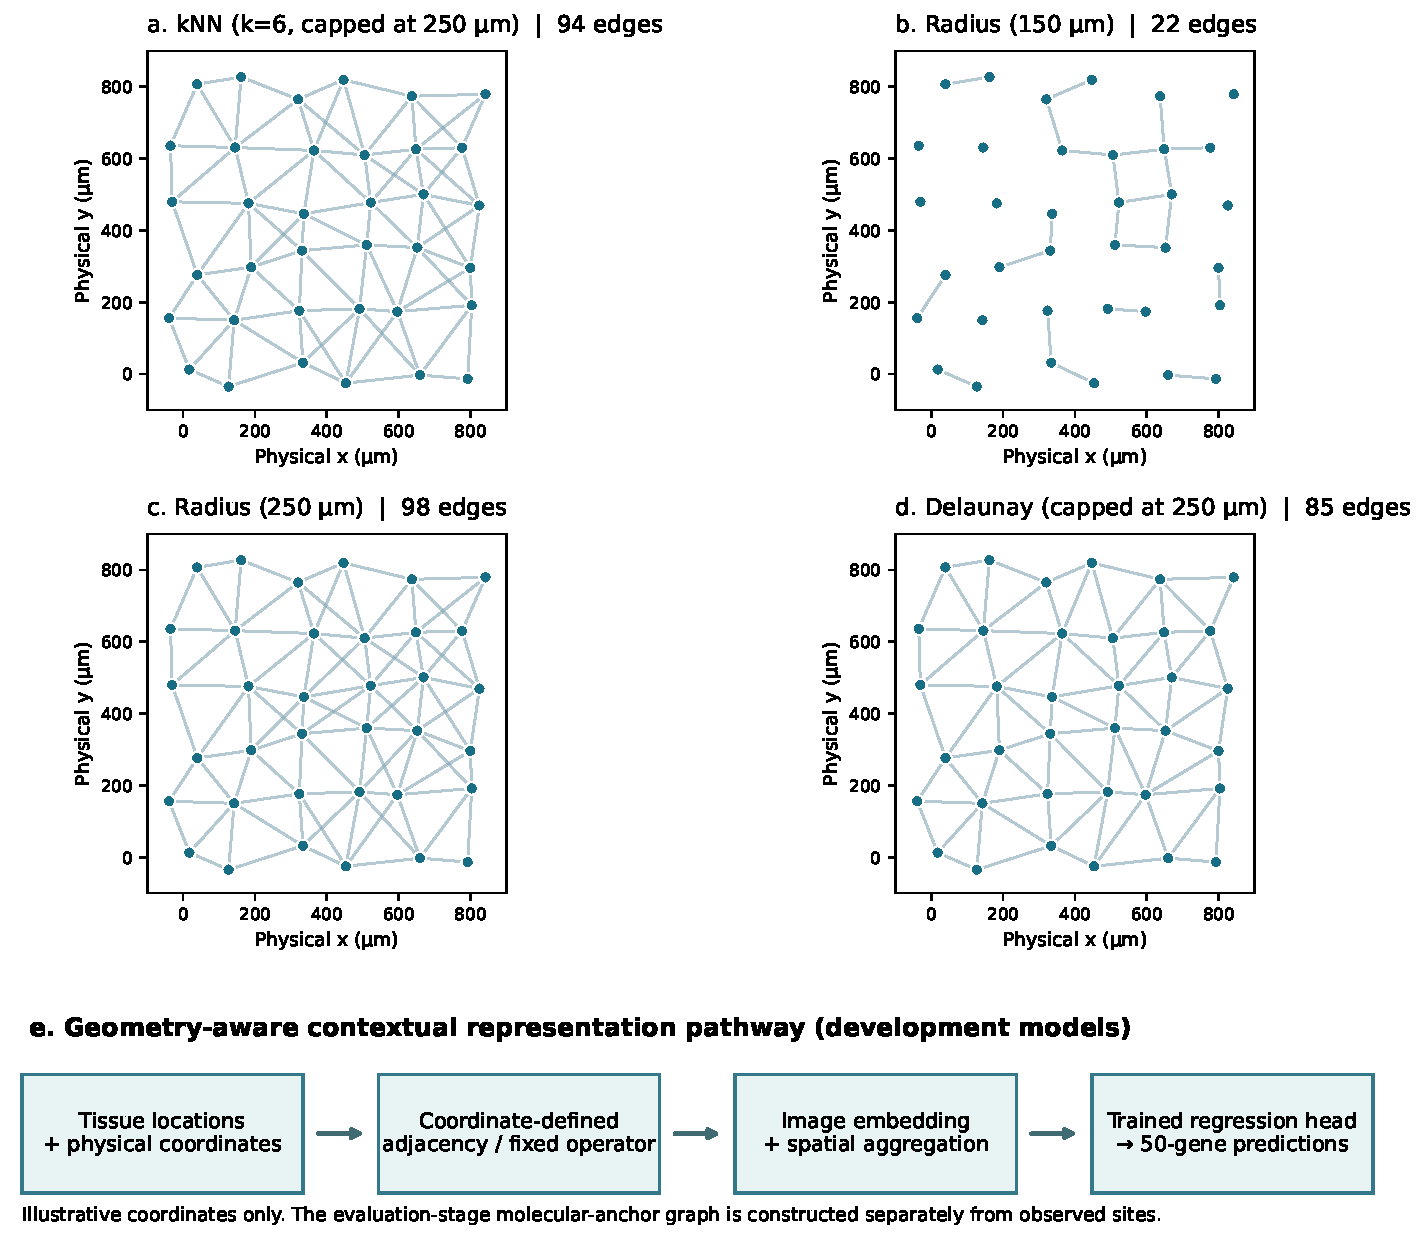
\includegraphics[width=\textwidth,height=0.78\textheight,keepaspectratio]{figures/Figure2.pdf}
\caption{\textbf{Geometry-aware graph construction and contextual representations.} \textbf{a--d,} The same 36 synthetic tissue locations are connected by (a) a symmetrized six-nearest-neighbor graph with a 250-\um{} distance cap, (b,c) 150- and 250-\um{} radius neighborhoods, or (d) a 250-\um{}-capped Delaunay graph. Coordinates and axes are identical across panels and all retained edges are displayed. Symmetrization means that a node can have more than six neighbors. \textbf{e,} Geometry determines a fixed adjacency/aggregation operator acting on the frozen image embeddings before an expression-regression head. The molecular-reconstruction stage uses a separate observation-dependent graph joining hidden locations to up to 16 measured molecular anchors. Synthetic points illustrate the architecture only, not a fitted patient graph or a performance result.}
\label{fig:graph_architecture}
\end{figure}